\documentclass{beamer}
%\documentclass{article}
%\usepackage{beamerarticle}
%\pagestyle{plain}
\newcommand{\bfX}{{\mbox{{\bf X}}}}
\newcommand{\bfR}{{\mbox{{\bf R}}}}

\usepackage{amssymb}
\usepackage{amsmath}
\newcommand\reals{\ensuremath{\mathbb{R}}}
%\newcommand{\bfX}{{\mbox{{\bf X}}}}
\newcommand{\bfY}{{\mbox{{\bf Y}}}}
\DeclareFontShape{OT1}{cmtt}{bx}{n}{
  <5><6><7><8><9><10><10.95><12><14.4><17.28><20.74><24.88>cmttb10}{}



\listfiles

\renewcommand\emptyset{\varnothing}
%\renewcommand\cdot{\mathop{\raise2pt\hbox{$\bullet$}}}
\renewcommand\cdot{\mathop{\raise-1pt\hbox{$^{_\bullet}$}}}

\renewcommand\today{November 21, 2017}
\title[cars.com and intro stats]{
Data scraping, ingestation, and modeling: bringing cars.com into the intro stats class}
\author{Nicholas J. Horton}
\institute{{\large Department of Mathematics and Statistics \\Amherst College, Amherst, MA, USA}}
\date{CAUSE webinar, \today}


\mode<presentation>
{
  \usetheme{Warsaw}
  %\usetheme{Copenhagen}
  % or ...

  %\setbeamercovered{transparent}
  % or whatever (possibly just delete it)
}

\AtBeginSubsection[]
{
  %\begin{frame}<beamer>
    %\frametitle{Outline}
    %\tableofcontents[currentsection,currentsubsection]
  %\end{frame}
}



\begin{document}
\frame{\titlepage
nhorton@amherst.edu \\
http://nhorton.people.amherst.edu, https://github.com/Amherst-Statistics/Cars-Scraping-Webinar}


\frame{
\frametitle{Thanks and acknowledgments}
\begin{itemize}
\item Danny Kaplan (for the original idea)
\item Project MOSAIC: Danny Kaplan (Macalester College), Randy Pruim (Calvin College), Ben Baumer (Smith College), and Johanna Hardin (Pomona College)
\item NSF \# 0920350
\end{itemize}
}

\frame{
\frametitle{Goal}
\begin{itemize}
\item I will describe a classroom activity where pairs of students hand scrape data from cars.com, ingest these data into R, then carry out analyses of the relationships between price, mileage, and model year for a selected type of car. 
\item This early in the semester activity can help illustrate the statistical problem solving process. 
\item The ``Less Volume, More Creativity" approach utilized by the mosaic package facilitates the analysis with a minimal amount of syntax. 
\item Key concepts that are introduced and reinforced including data ingestion, multivariate thinking through graphical visualizations, and regression modeling. 
\item Extensions and additional use of the dataset will be discussed along with potential pitfalls.
\end{itemize}
}

\frame{
\frametitle{Cars, cars, and more cars}
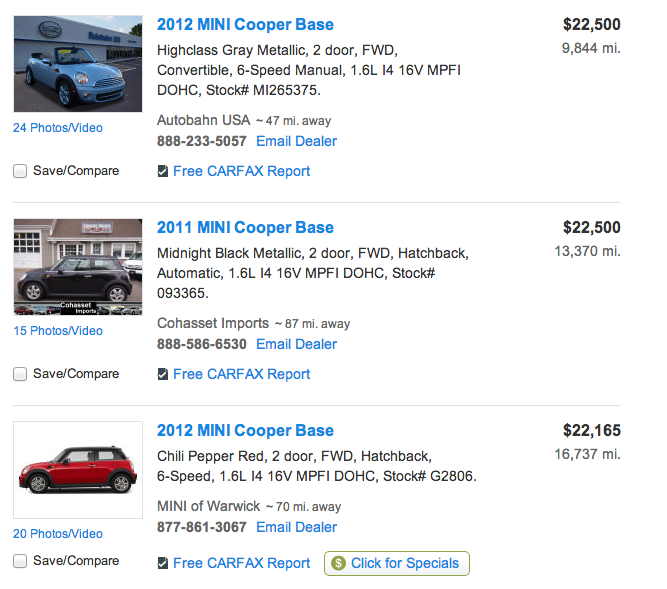
\includegraphics[scale=0.52]{images/cars.png}
}

\frame{
\frametitle{Questions?}
\begin{itemize}
\item How much do cars cost?
\item How much do car prices vary?
\item How are car prices associated with mileage?
\item How are car prices associated with age?
\item How quickly do new cars depreciate?
\item How much does it cost for a car to drive a mile?
\end{itemize}
}

\frame{
\frametitle{revised GAISE College report}

\includegraphics[scale=0.28]{gaise}}

\frame{
\frametitle{revised GAISE College Report (2016)}
\begin{enumerate}
\item Teach statistical thinking.
\begin{itemize}
\item Teach statistics as an investigative process of problem-solving and decision-making.
\item Give students experience with \emph{multivariable thinking}.
\end{itemize}
\item Focus on conceptual understanding.
\item Integrate real data with a context and purpose.
\item Foster active learning.
\item Use technology to explore concepts and analyze data.
\item Use assessments to improve and evaluate student learning.
\end{enumerate}
}

\frame{
\frametitle{Motivation for multivariate thinking}
\begin{itemize}
\item We live in a multivariate world
\item If intro stats only addresses bivariate questions (e.g., two-sample t-test) we risk becoming irrelevant
\item Straightforward to consider multivariate visualizations
and fit multiple regression models (Project MOSAIC ``Less Volume, More Creativity")
\item \emph{R Journal}: \url{https://journal.r-project.org/archive/2017/RJ-2017-024}
\end{itemize}
}

\frame{
\frametitle{Cars.com Activity}
\begin{description}
\item[Groups] of size two
\item[Duration] one or two 50-minute class periods
\item[Requirements] one computer per student
\item[Software] R/RStudio and Excel or Open Office
\item[Motivation] Why might we care about car prices?
\end{description}
}

\frame{
\frametitle{Cars.com Activity}
\begin{description}
\item[Group] is given a major city in the US (e.g., Atlanta or Los Angeles)
\item[Person 1] searches \url{cars.com} for used Toyota Prius cars on offer within 50 miles of that city
\item[Person 2] downloads the template {\tt cars.csv} spreadsheet and open it up on their computer
\item[Person 1] reads out car models, year, mileage, and price
\item[Person 2] enters the values into the spreadsheet and reads them out for Person 1 to check
\item[Continue] until 40 cars have been entered (note that some groups will be really slow, so may only yield 20-25 cars)
\item[Person 2] emails Person 1 the {\tt cars.csv} spreadsheet then both members upload this into RStudio
\end{description}
}

\frame{
\frametitle{Cars.com analysis (part 1)}
\begin{itemize}
\item The file {\tt student.Rmd} reads {\tt cars.csv}
\item Generates descriptive statistics (for data quality assessment, e.g., using \$ in price)
\item Create visual multivariate displays (e.g., mileage by year)
\item Fit regression model and display coefficients
\end{itemize}
}

\frame{
\frametitle{Cars.com analysis (part 2)}
\begin{itemize}
\item Once {\tt student.Rmd} runs without error, the creative step begins
\item Students need to find an interesting display and fit a multiple regression model
\item Goal is to make an insight
\item Publish this on \url{rpubs.com} using a class-wide login provided by the instructor
\item Quickly review several of these to see insights
\item Deliverable: full credit for email to instructor (cc-ed to group partner) of modified {\tt student.Rmd} and {\tt cars.csv} files
\end{itemize}
}

\frame{
\frametitle{Examples}
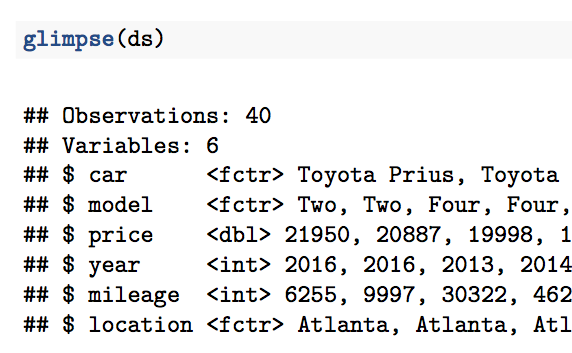
\includegraphics[scale=0.52]{images/cars-glimpse.png}
}
\frame{
\frametitle{Examples}
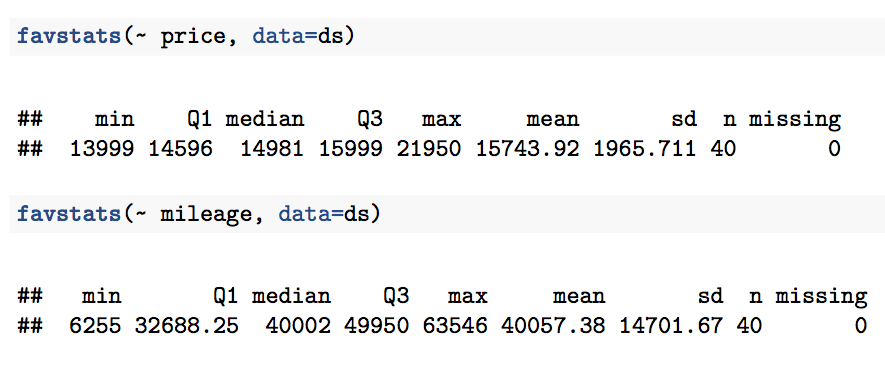
\includegraphics[scale=0.42]{images/cars-favstats.png}
}
\frame{
\frametitle{Examples}
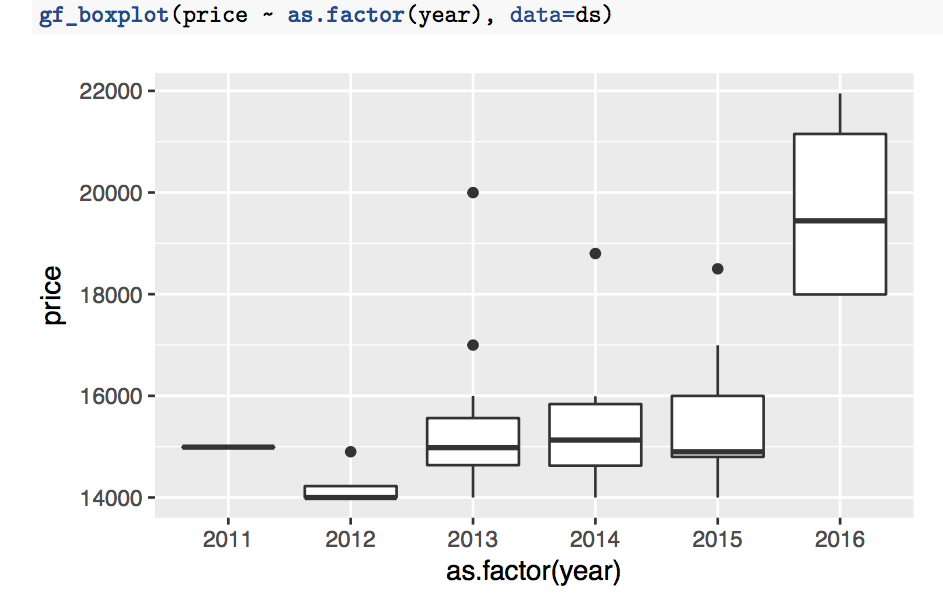
\includegraphics[scale=0.35]{images/cars-box.png}
}
\frame{
\frametitle{Examples}
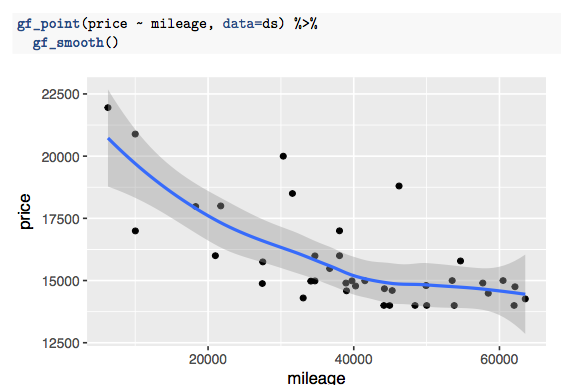
\includegraphics[scale=0.52]{images/cars-scat.png}
}

\frame{
\frametitle{Cars.com followup (next class)}
\begin{itemize}
\item Collate individual group data into {\tt carscollated2017.csv}
\item Perform data cleaning (e.g., numeric zip code rather than city)
\item Add location to the multiple regression model
\item Practice interpreting regression models with categorical predictors
\item Practice interpreting regression models with interactions between mileage and year
\item Seek insights: depreciation dramatic for new cars
\end{itemize}
}

\frame{
\frametitle{Tom and Ray Magliozzi}
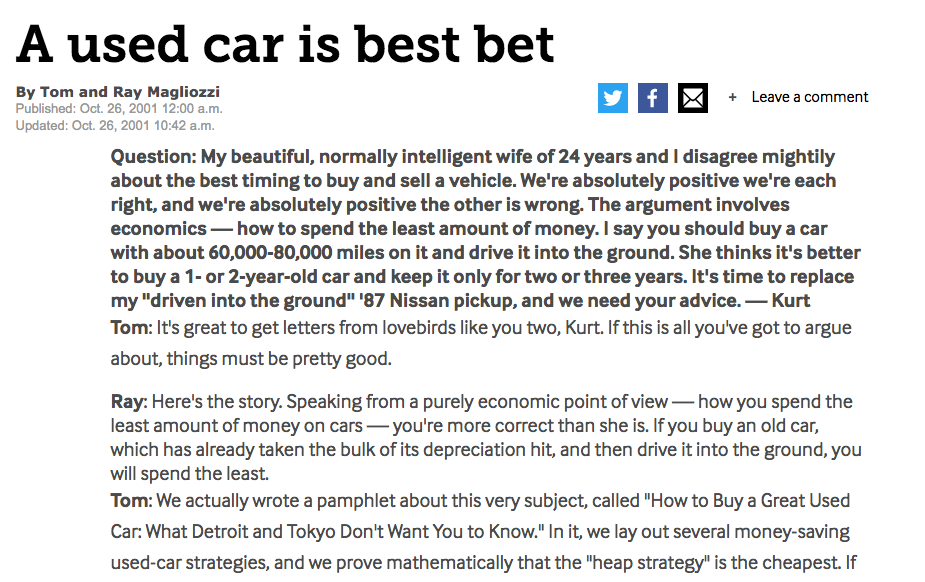
\includegraphics[scale=0.39]{images/magliozzi.png}
}

\frame{
\frametitle{Cars.com followup}
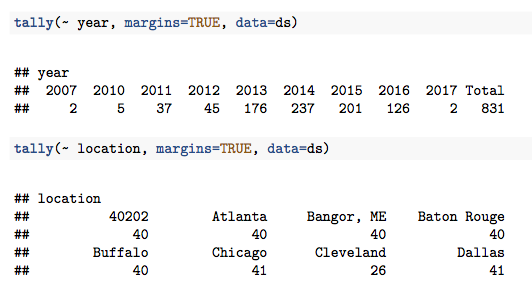
\includegraphics[scale=0.64]{images/cars-tally.png}
}

\frame{
\frametitle{Cars.com followup}
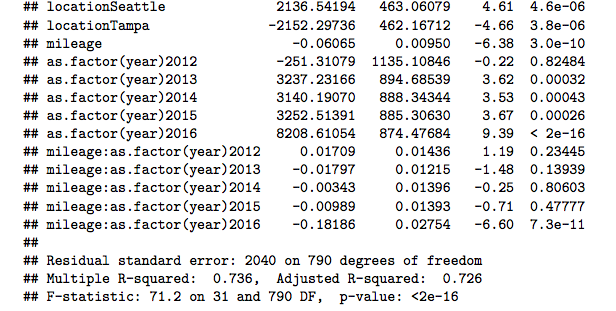
\includegraphics[scale=0.74]{images/cars-reg.png}
}

\frame{
\frametitle{Cars.com followup}
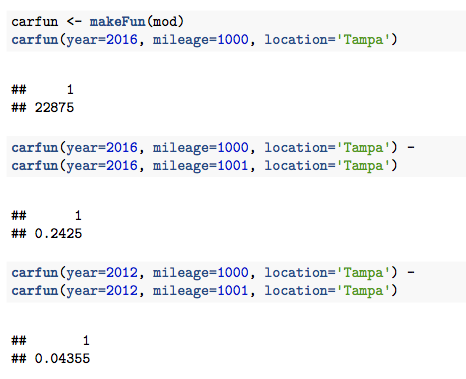
\includegraphics[scale=0.63]{images/cars-fun.png}
}

\frame{
\frametitle{Cars.com followup}
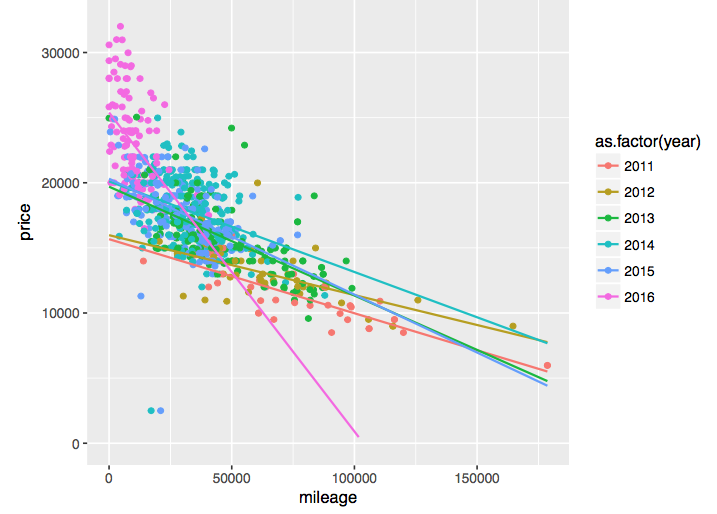
\includegraphics[scale=0.47]{images/cars-fin.png}
}

\frame{
\frametitle{Extension}
\begin{itemize}
\item Interpreting model is a great exam question
\item Residual diagnostics
\item Outlier detection
\item Account for different car models (sparsity and inconsistent coding)
\item Automate data scraping
\end{itemize}
}


\frame{
\frametitle{Closing thoughts}
\begin{itemize}
\item Ensure that students see multivariate examples early and often
\item Ensure that students use real tools
\item Once they have some experience with ``tame data", have them ingest their own
\item Motivate automated data scraping procedures
\item Practice composing and answering questions with data
\end{itemize}
}

\frame{\titlepage
nhorton@amherst.edu \\
http://nhorton.people.amherst.edu, https://github.com/Amherst-Statistics/Cars-Scraping-Webinar}

\end{document}
